\documentclass{article}

\usepackage[utf8]{inputenc} % For encoding
\usepackage{graphicx} % For including images
\usepackage{amsmath} % For mathematical formulas
\usepackage{biblatex} % For bibliography management
\usepackage{float} % For fixing the position of tables/figures

\addbibresource{references.bib} % Add your bibliography file here

\title{Microwave Experiment}
\author{Chen En, Ho}
\date{\today}

\begin{document}

\maketitle

\begin{abstract}
This is the abstract where you provide a brief summary of the document.
\end{abstract}

\section{Introduction}
In this section, you will introduce the topic and provide the background or motivation for your study.

\section{Methodology}
Here, describe the methods and approaches you used in your research or study.

\section{Experimental Apparatus}
This section includes the description of the experimental setup and apparatus you used in your work.

\section{Results \& Discussions}



The table below presents the data for \( V_{\text{peak-low}} \) and \( \frac{1}{4} \lambda \), along with the calculated mean and uncertainties for \( \lambda \)\footnote{In this article, the uncertainties consist of both Type A and Type B uncertainties. The total uncertainty is calculated using error propagation.}.

\begin{table}[H]
    \centering
    \begin{tabular}{|c|c|c|}
        \hline
        \( V_{\text{peak-low}} \) & \( V_{\text{peak-low}} \) & \( \frac{1}{4} \lambda \) (mm) \\
        \hline
        157 & 147.5 & 9.5 \\
        147.5 & 137 & 10.5 \\
        137 & 124 & 13 \\
        124 & 113.5 & 10.5 \\
        113.5 & 101.5 & 12 \\
        101.5 & 91.5 & 10 \\
        91.5 & 79.9 & 11.6 \\
        \hline
    \end{tabular}
    \caption{Values of \( V_{\text{peak-low}} \) and corresponding \( \frac{1}{4} \lambda \).}
\end{table}

Therefore, the wavelength \( \lambda \) with its total uncertainty is:

\[
\lambda = 0.04406 \, \text{m} \pm 0.00186 \, \text{m} \quad (4.23\%)
\]

Then, a relationship between the intensity $I$ and the distance from a node $d$ is measured. 

\begin{table}[H]
    \centering
    \begin{tabular}{|c|c|c|c|}
        \hline
        I ($\nu$A) & \( I \) (A) & d (mm) & \( \bar{d} \) (m) \\
        \hline
        -0.0025 & -2.7E-09 & 136.9 & 1E-04 \\
        -0.0027 & 1.2E-08 & 137 & 0.0011 \\
        0.012 & 3.75E-08 & 138 & 0.0021 \\
        0.0375 & 8.58E-08 & 139 & 0.0031 \\
        0.0858 & 1.216E-07 & 140 & 0.0041 \\
        0.1216 & 1.698E-07 & 141 & 0.0051 \\
        0.1698 & 2.264E-07 & 142 & 0.0061 \\
        0.2264 & 2.792E-07 & 143 & 0.0071 \\
        0.2792 & 3.178E-07 & 144 & 0.0081 \\
        0.3178 & 3.54E-07 & 145 & 0.0091 \\
        0.354 & 3.636E-07 & 146 & 0.01081 \\
        0.3636 & & 147.71 & \\
        \hline
    \end{tabular}
    \caption{Values of \( I (\nu A) \), \( I \, \text{(A)} \), \( d \, \text{(mm)} \), and \( \bar{d} \, \text{(m)} \).}
\end{table}

If we plot $I$ versus $sin(2\pi d/\lambda_g)$, we found that the result is close to a exponential graph (except the last data).

\begin{figure}[H]
    \centering
    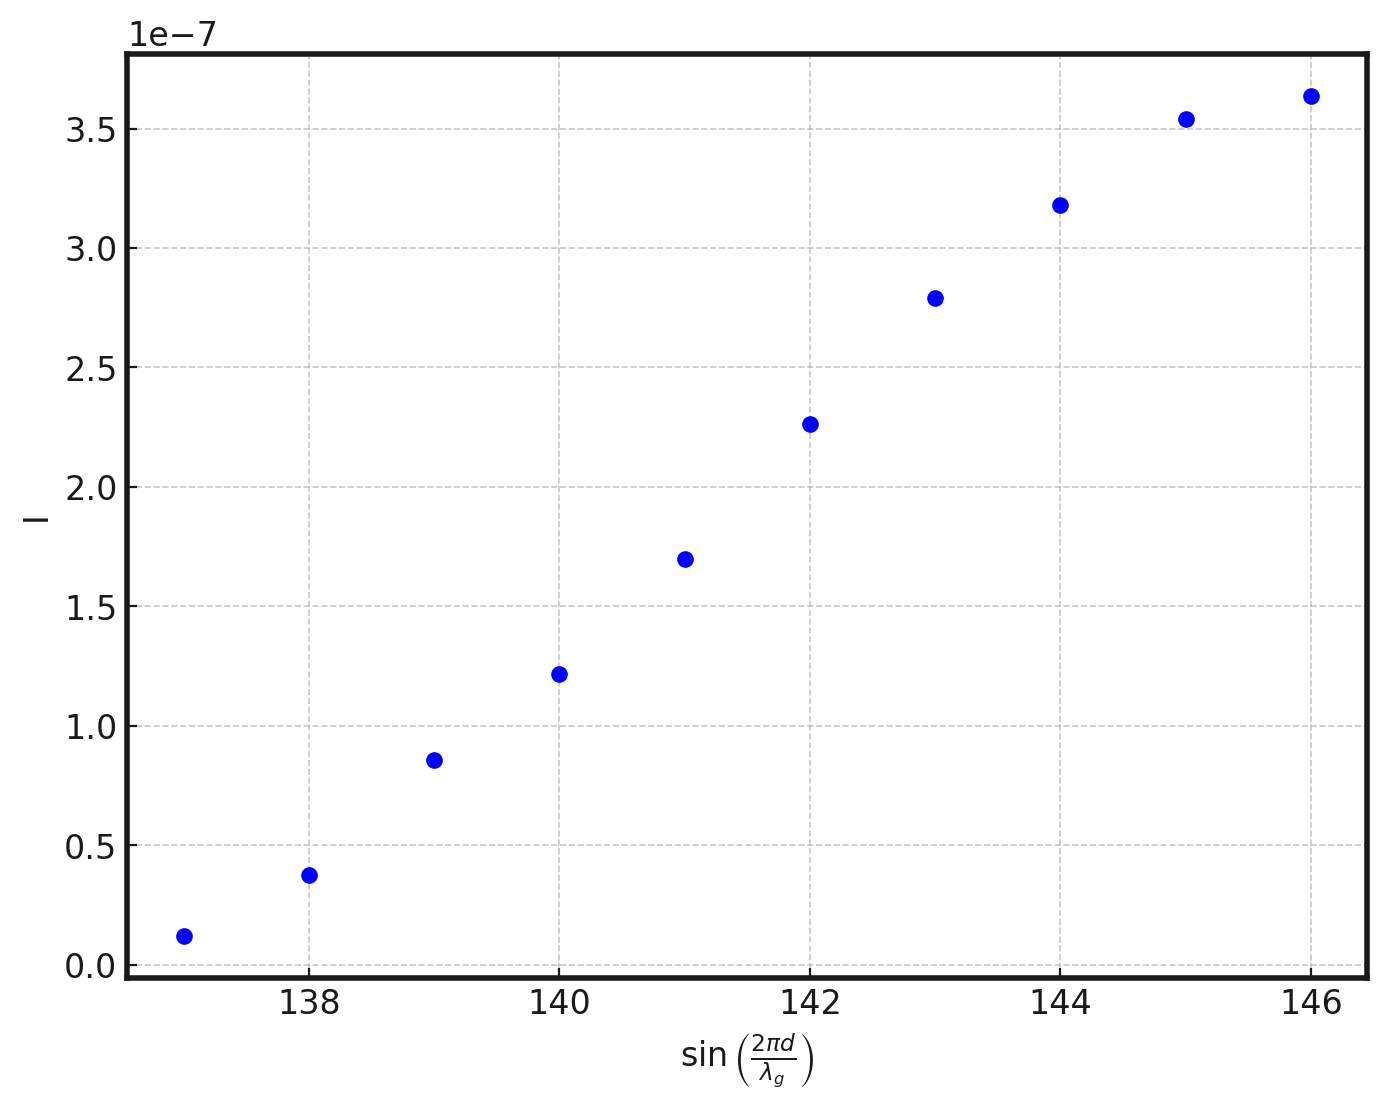
\includegraphics[width=0.8\textwidth]{./media/lab1 raw I-V.png}
    \caption{ $I$(A)-$sin(2\pi d/\lambda_g$) characteristics from the experiment.}
    \label{fig:raw_iv}
\end{figure}

Hence, we can guess $I=C\cdot sin(\frac{2\pi d}{\lambda_g})^n$. A linear regression analysis was conducted. 

\begin{figure}[H]
    \centering
    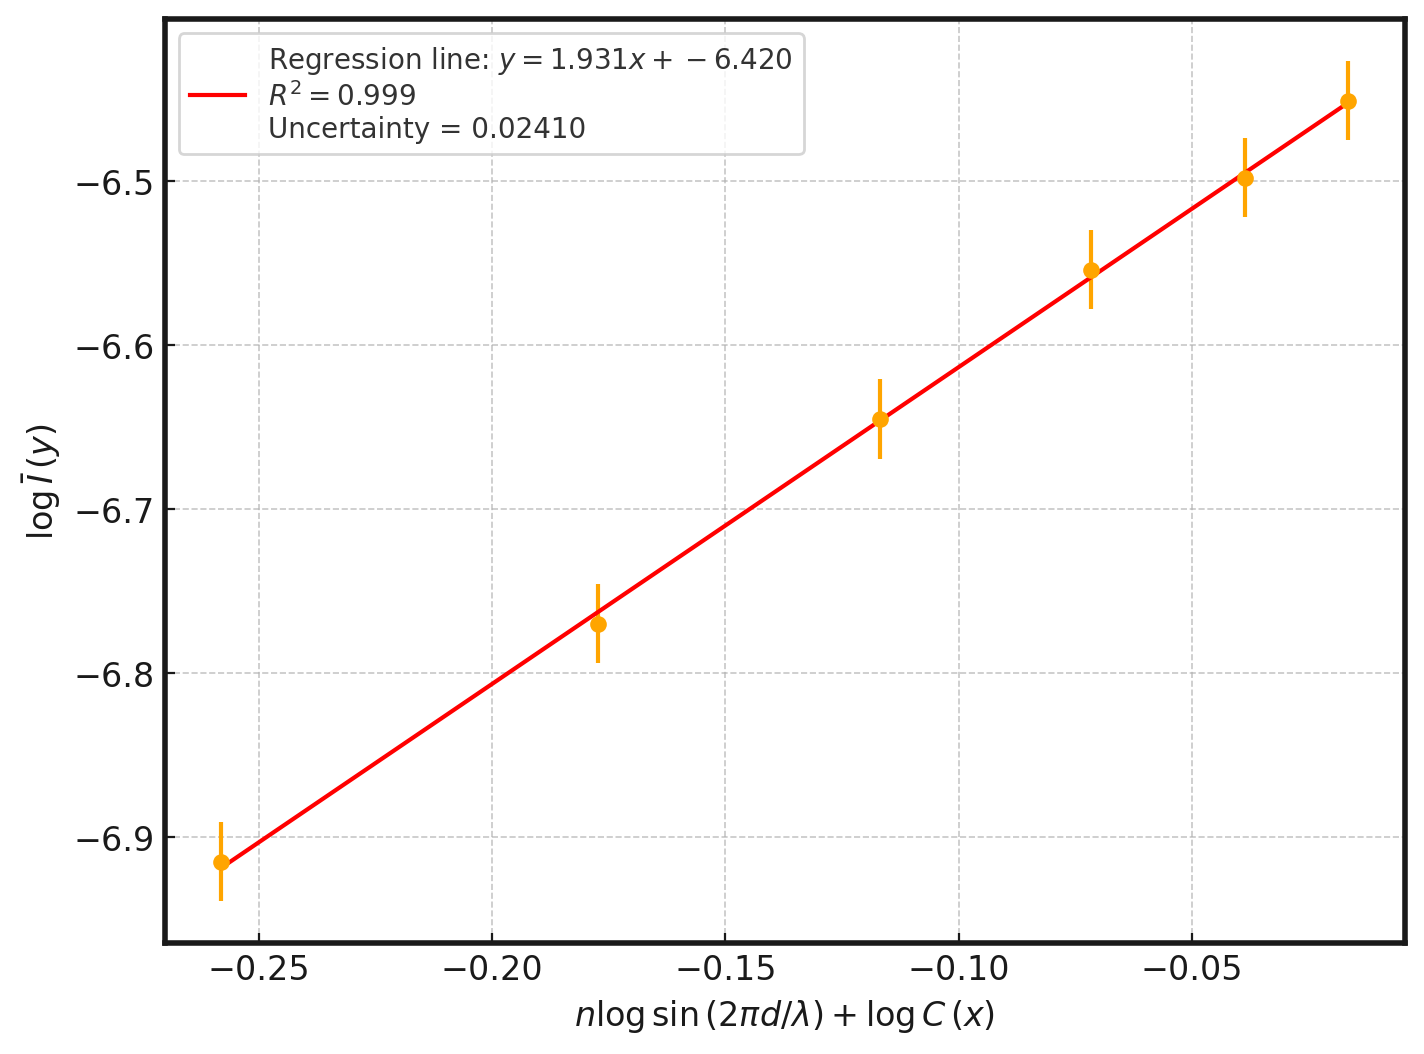
\includegraphics[width=0.9\textwidth]{./media/lab1.png}
    \caption{Linear regression analysis of $\log \bar{I}$ vs $n \log \sin\left(2 \pi d / \lambda \right) + \log C$.}
    \label{fig:regression}
\end{figure}

we get:

\[
n = 1.931 \pm 0.024 \quad (1.24\%)
\]



\section{Textbook Questions}
Here, include any questions from textbooks or exercises that are relevant to your topic.

\section{Conclusion}
Summarize the main findings and key points from the study.

\printbibliography

\end{document}
